% Auto-generated paper tables and figures
% Run: python scripts/generate_paper_tables.py --results-dir results

\usepackage{booktabs}
\usepackage{graphicx}
\usepackage{tikz}
\usepackage{pgfplots}
\pgfplotsset{compat=1.18}

\textbf{Table 1: Internal LegalQA} — Data not available.

\begin{table}[t]
\centering
\caption{External VLegal Paired Benchmark. Base vs.~QLoRA on identical samples.}
\label{tab:external}
\begin{tabular}{lclcc}
\toprule
Task & N & Metric & Base & QLoRA & $\Delta$ (95\% CI) \\
\midrule
Article Clause Prediction & 20 & accuracy & 0.5500 & 0.5500 & +0.0000 [+0.000, +0.000] \\
Court Decision Prediction & 20 & accuracy & 0.5500 & 0.5500 & +0.0000 [+0.000, +0.000] \\
Multi Hop Reasoning & 20 & accuracy & 0.2500 & 0.2500 & +0.0000 [+0.000, +0.000] \\
Penalty Remedy Estimation & 20 & token_f1 & 0.0510 & 0.0510 & +0.0000 [+0.000, +0.000] \\
\bottomrule
\end{tabular}
\vspace{1mm}
\parbox{0.9\textwidth}{\footnotesize $^*$ $p < 0.05$; CI via paired bootstrap (1000 resamples).}
\end{table}

\begin{table}[t]
\centering
\caption{Capability Transfer: Internal $\to$ External (valid mappings only).}
\label{tab:capability}
\begin{tabular}{llccc}
\toprule
Internal Capability & External Task & Base & QLoRA & $\Delta$ \\
\midrule
Reasoning/Inference & Article Clause Prediction & 0.5500 & 0.5500 & +0.0000 \\
 & Court Decision Prediction & 0.5500 & 0.5500 & +0.0000 \\
 & Multi Hop Reasoning & 0.2500 & 0.2500 & +0.0000 \\
 & Penalty Remedy Estimation & 0.0510 & 0.0510 & +0.0000 \\
\bottomrule
\end{tabular}

\vspace{1mm}
\parbox{0.9\textwidth}{\footnotesize Only capability-task pairs with clear semantic alignment are included. Categories without external counterparts (Ethics/Bias, NER, RE) are marked N/A.}
\end{table}

\textbf{Table 4: Evidence Degradation} — No results.

\textbf{Table 5: Evidence Sensitivity} — No results.


% Figure 1: Internal gain vs External gain
\begin{figure}[t]
\centering
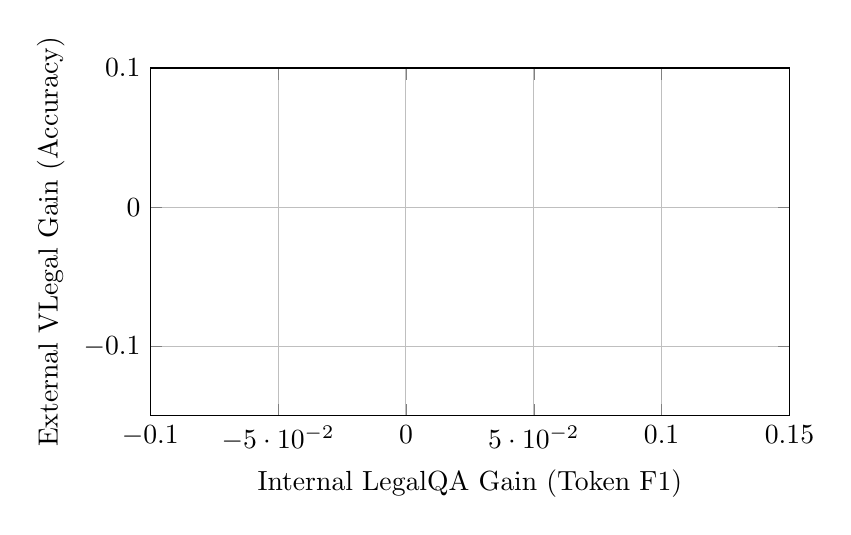
\begin{tikzpicture}
\begin{axis}[
    width=0.8\textwidth,
    height=6cm,
    xlabel={Internal LegalQA Gain (Token F1)},
    ylabel={External VLegal Gain (Accuracy)},
    xmin=-0.1, xmax=0.15,
    ymin=-0.15, ymax=0.1,
    grid=major,
    legend pos=south west,
]
% Add data points from paired benchmark results
% \addplot[only marks, mark=*, color=blue] coordinates {
%   (internal_delta_1, external_delta_task_1)
%   ...
% };
% \addlegendentry{Task}
\end{axis}
\end{tikzpicture}
\caption{Internal LegalQA gain vs.\ external VLegal gain after QLoRA adaptation. Points below zero on the y-axis indicate specialization--generalization trade-off.}
\label{fig:internal_vs_external}
\end{figure}


% Figure 2: Evidence degradation curve
\begin{figure}[t]
\centering
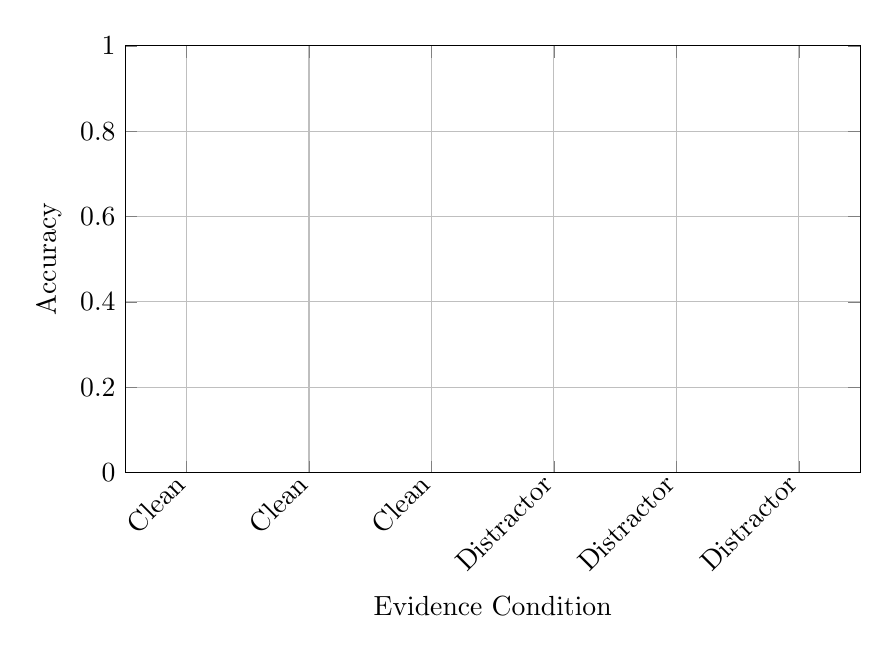
\begin{tikzpicture}
\begin{axis}[
    width=0.9\textwidth,
    height=7cm,
    xlabel={Evidence Condition},
    ylabel={Accuracy},
    symbolic x coords={Clean, Distractor, Miss. Rule, Miss. Cond., Miss. Exc., Wrong-Sim., Empty, Shuffled},
    xtick=data,
    x tick label style={rotate=45, anchor=east},
    ymin=0, ymax=1,
    grid=major,
    legend pos=north east,
    mark size=2pt,
]
% Base model line
% \addplot[mark=square*, color=red] coordinates { ... };
% \addlegendentry{Base}
% QLoRA model line
% \addplot[mark=triangle*, color=blue] coordinates { ... };
% \addlegendentry{QLoRA}
\end{axis}
\end{tikzpicture}
\caption{Evidence degradation curve: Base vs.\ QLoRA across 8 evidence conditions. A flat QLoRA line suggests reduced evidence sensitivity.}
\label{fig:degradation}
\end{figure}
